\documentclass{beamer}
%\usetheme{default}

\usetheme{JuanLesPins}
\usepackage{listings}
\usepackage{times}

%\usepackage{xkeyval}
\usefonttheme{structurebold}

\usepackage[english]{babel}
%\usepackage{pgf,pgfarrows,pgfnodes,pgfautomata,pgfheaps,graphics}\usepackage{pgflibraryshapes}
%\usepackage{graphics}
\usepackage{epsfig}
\usepackage{amsmath,amssymb}
\usepackage[latin1]{inputenc}


%%%%%%%%%%%%%%CARDIS%%%%%%%%%%%%%%%%%%%%%%

\usepackage{tikz}
\usepackage{graphics}
\usepackage{pgflibraryshapes}

\usepackage{listings}

\lstset{escapeinside={(*@}{@*)}}
\lstset{commentstyle=\color{blue!50!black}\textit,tabsize=2,keywordstyle=\color{green!50!black}}
\lstset{backgroundcolor=\color{lightgray!50}}
%\lstset{frame=trbl,frameround=DDDD}
\lstset{numbers=left, numberstyle=\footnotesize}

\usepackage{multirow}
\newcommand{\benchname}[1]{\texttt{#1}}


\setbeamercovered{dynamic}
%\beamertemplatenavigationsymbolsempty

\title[]{Java bytecode specification and verification}
\author[mariela.pavlova@sophia.inria.fr]{\textbf{Mariela Pavlova}}
\date[CARDIS'06]{Seventh Smart Card Research and Advanced Application IFIP Conference, April 19th, 2006}
\date[INRIA Sophia Antipolis ]{Supervisors Gilles Barthe and Lilian Burdy}

\AtBeginSection[]{\frame{\frametitle{Outline}\tableofcontents[current]}}

\begin{document}

\begin{frame}
\titlepage
\end{frame}

%\newcommand{\stack}[1]{\mbox{\rm\textbf{st}}(#1)}% element on top stack 
%\newcommand{\counter}{\mbox{\rm\textbf{c}}}
%\newcommand{\locVar}[1]{\mbox{\rm{\textbf{reg}}}(#1) }


\newcommand{\LST}{\ensuremath{\mathsf{G}}}
\newcommand{\MST}{\ensuremath{\mathsf{M}}}
\newcommand{\Anno}{\ensuremath{\mathsf{Q}}}

\newcommand{\JudgeF}[4]{\ensuremath{\LST,\Anno \vdash \lbrace {#2} \rbrace\, {#1}\, \lbrace {#3} \rbrace\, ({#4})}}

\newcommand{\ppt}{\ensuremath{\mathit{pc}}}


\newcommand{\sem}[1]{\ensuremath{[\![{#1}]\!]_{\small{\textit{BML}}}\/}}

\newcommand{\mobius}{\textsf{MOBIUS}\xspace}

\newcommand{\varHook}[1]{\mbox{\slshape #1}}
\newcommand{\codeHook}[1]{\mbox{\ttfamily #1}}



%%%%%%%%%%%%%%%%%%%%%%%%%%%%%%%%%%%%%%%%%%%%%%%%%%%%%%%%%%%%%%%%%%%%%%%%%%%%%%%%%%%%%%%%%%%%%%%%%%%%%%
%%%%%%%%%%%%%%%%%%%%%%%%%%%%%%%%%%%%%%%%BYTECODE LANGUAGE%%%%%%%%%%%%%%%%%%%%%%%%%%%%%%%%%%%%%%%%%%%%%%%%%%%
%%%%%%%%%%%%%%%%%%%%%%%%%%%%%%%%%%%%%%%%%%%%%%%%%%%%%%%%%%%%%%%%%%%%%%%%%%%%%%%%%%%%%%%%%%%%%%%%%%%%%%%%%%%%
% \newcommand{\bcIns}{\mbox{ \rm I} }
% \newcommand{\instrs}{\mbox{ \rm IS} }
% \newcommand{\ifCond}{ \instr{if\_cond } }
% \newcommand{\goto}{ \instr{goto } }
% \newcommand{\return}{ \instr{return } }
% \newcommand{\arithOp}{ \instr{arith\_op} }
% \newcommand{\load}{ \instr{load} }
% \newcommand{\store}{ \instr{store} }
% \newcommand{\push}{ \instr{push} }
% \newcommand{\pop}{\instr{pop}}
% \newcommand{\dup}{\instr{dup}}
% \newcommand{\iinc}{\instr{iinc}}
% \newcommand{\new}{\instr{new}}
% \newcommand{\newarray}{\instr{newarray}}
% \newcommand{\putfield}{\instr{putfield}} 
% \newcommand{\getfield}{\instr{getfield}}
% \newcommand{\arrstore}{\instr{type\_astore}} 
% \newcommand{\arrload}{\instr{type\_aload}}
% \newcommand{\arraylength}{\instr{arraylength}}
% \newcommand{\instanceof}{\instr{instanceof}} 
% \newcommand{\checkcast}{\instr{checkcast}} 
% \newcommand{\athrow}{\instr{athrow}}
% \newcommand{\invoke}{\instr{invoke}}
% \newcommand{\jsr}{\instr{jsr}}
% \newcommand{\ret}{\instr{ret}}
% \newcommand{\swap}{\instr{swap}}
%%%%%%%%%%%%%%%%%%%%%%%%%%%%%%%%%%%%%%%%%%%%%%%%%%%%%%%%%%%%%%%%%%%%%%%%%%%%%%%%%%%%%%%%%%%%%%%%%%%%%%
%%%%%%%%%%%%%%%%%%%%%%%%%%%%%%%%%%%%%%%%BYTECODE LANGUAGE%%%%%%%%%%%%%%%%%%%%%%%%%%%%%%%%%%%%%%%%%%%%%%%%%%%
%%%%%%%%%%%%%%%%%%%%%%%%%%%%%%%%%%%%%%%%%%%%%%%%%%%%%%%%%%%%%%%%%%%%%%%%%%%%%%%%%%%%%%%%%%%%%%%%%%%%%%%%%%%%



\newcommand{\todo}[1]{\marginpar{\baselineskip0ex\rule{2,5cm}{0.5pt}\\[0ex]{\textsf{#1}}}}
%\newcommand{\fig}[1]{ Fig.#1}
\newcommand{\jmlKey}[1]{\texttt{#1}}% wrapping jml keywords
%\newcommand{\java}[1]{\texttt{#1}}
%\newcommand{\stack}[1]{\mbox{\rm\textbf{st}}(#1)}% element on top stack 
%\newcommand{\stackOnly}{\mbox{\rm St}}
%\newcommand{\stackOnlyParam}[1]{\mbox{\rm St}(#1)}
%\newcommand{\newStack}{ \lbrack~\rbrack  } % empty stack
%\newcommand{\update}[3]{ #1 [ \oplus {#2} \rightarrow {#3} ] }

%\newcommand{\counter}{\mbox{\rm\textbf{cntr}} }
%\newcommand{\counterOnly}{\mbox{\rm Cntr} }
%\newcommand{\topStack}{\mbox{\rm cntr} }
%\newcommand{\true}{\mbox{\rm\textbf{true}} } % true from the assertion language
%\newcommand{\false}{\mbox{\rm\textbf{false}}} % false from the assertion language



%\newcommand{\instr}[1]{\mbox{  \rm #1} }

%\newcommand{\loopStart}[1]{\textbf{loop\_start$\tt{_#1}$}}
%\newcommand{\loopEnd}[1]{\textbf{loop\_end$\tt{_#1}$}}
%\newcommand{\invariant}[1]{\it{I}_{\tt{#1}}}
%\newcommand{\boucle}[1]{\texttt{#1}}
%\newcommand{\loopModifies}[1]{\textbf{Modifies}(\texttt{#1}) }
%\newcommand{\ins}[1]{#1 : \mbox{\rm\texttt{instr}}}


%\newcommand{\insOnly}{\texttt{instr}}

% the grammar for the bytecode specification language
%\newcommand{\ClassSpec}{\rm{ClassSpec}}
%\newcommand{\ClassInv}{ClassInv}
%\newcommand{\ClassHistoryConstr}{ClassHistoryConstr}

%\newcommand{\MethodSpec}{\rm{MethodSpec}}


%\newcommand{\specCase}{\textrm{SpecCase}}
%\newcommand{\requires}{requires}
%\newcommand{\ensures}{ensures}
%\newcommand{\exsures}{exsures}
%\newcommand{\modifies}{modifies}

%\newcommand{\jmlStmt}[1]{\textrm{#1}}
%\newcommand{\specExpression}{\mathcal{E}^{spec}}

%\newcommand{\interMethodSpec}{\rm{InterMethodSpec}}
%\newcommand{\loopSpec}{\rm{loopSpec}}
%\newcommand{\assert}{\rm{assert}}

%\newcommand{\ArithExpr}{\texttt{ArithmeticExp} }

%\newcommand{\JMLExpr }{\texttt{JmlExp} }


%\newcommand{\integer}{\texttt{int} }
%\newcommand{\register}[1]{\mbox{\rm\textbf{reg}}(#1)}

%\newcommand{\Mynull}{\jmlKey{null}}
%%\newcommand{\this}{\texttt{this}}
\newcommand{\fieldAccess}[2]{#1\texttt{.}#2}
\newcommand{\arrayAccess}[2]{\texttt{arrayAccess(} #1 \texttt{,} #2\texttt{)}}  
%\newcommand{\arrayAccessOnly}{\mbox{\rm arrAccess}}


%\newcommand{\loopInv}{loopInvariant}
%\newcommand{\loopMod}{loopModifies}

\newcommand{\result}{\jmlKey{\bsl result}}
%\newcommand{\old}[1]{\jmlKey{$\backslash$old(}#1\jmlKey{)}}
%\newcommand{\typeof}[1]{\jmlKey{$\backslash$typeof(}#1 \jmlKey{)}}
%\newcommand{\TYPE}{\jmlKey{TYPE} }
%\newcommand{\elemtype}[1]{ \jmlKey{$\backslash$elemtype(}#1\jmlKey{)} } 
%\newcommand{\excPost}{\psi^{exc}}

%\newcommand{\Myspace}{\phantom{aaa}}
%\newcommand{\predicate}{ \mathcal{P}} 
%\newcommand{\Myfalse}{ \textit{false} }
%\newcommand{\Mytrue}{ \textit{true} }



%% abstractCtrlFlow.tex
%\newcommand{\execRel}{\rightarrow} % the execution relation
%\newcommand{\blockm}[1]{ \tt{b^{#1}} }
%\newcommand{\blockSeq}[1]{ \tt{b_{seq}^{#1}} }
%\newcommand{\pathm}[2]{\blockm{#1} \execRel^{*} \blockm{#2} }
%\newcommand{\instrPost}[1]{ post(\instr{#1} )}





%from wp.tex
%\newcommand{\wpExeWithLoops}[1]{ \rm{Wp''}\rm{(#1)} }
%\newcommand{\wpExe}[1]{ \rm{Wp'}\rm{(#1)} }



%\newcommand{\getExcPost}{\mbox{\rm\textsf{getExcPostIns}}}
%\newcommand{\excPost}{\mbox{\rm\textsf{excPost}}}
%\newcommand{\javaNull}{null}
%\newcommand{\length}{\mbox{\rm arrLength}} % stands for array length


%%%%%%%%%%%%%%%%%%%%%%%%%%%%%%%%%%%%%%%%%%%%%%%%%%%%%%%%%%%%%%%%%%%%%%%%%%%%%%%%%%%%%%%%%%%%%%%%%%%%%%%%%%%%%%%%%%%%%%%%%%%%%%%%%%%%%%%%%%%%%%%%%%%%%%%%%%%%%%%%%%%%%%%%%%%%%%%%%%%%%%%%%%%%%%%%%%%%%%%%%%%%%%%%%%%%%%%%%%%%%%%%%%%%%%%%%%%%%%WP functions%%%%%%%%%%%%%%%%%%%%%%%%%%%%%%%%%%%%%%%%%%%%%%%%%%%%%%%%%%%%%%%%%%%%%%%%%%%%%%%%%%%%%%%%%%%%%%
%%%%%%%%%%%%%%%%%%%%%%%%%%%%%%%%%%%%%%%%%%%%%%%%%%%%%%%%%%%%%%%%%%%%%%%%%%%%%%%%%%%%%%%%%%%%%%%%%%%%%%%%%%%%%%%%%%%%%%%%%%%%%%%%%%%%%%%% 

%\newcommand{\wpi}[3]{\mbox{\rm\textit{wp}}(#3 \  #1, #2) }
%\newcommand{\fwpi}{\mbox{\rm\textit{wp}}}
%\newcommand{\inter}[2]{\mbox{ \rm \textit{inter}}(#1, #2, \methodd)} % predicate that holds between two bytecode blocks
%\newcommand{\interOnly}{\mbox{ \rm \textit{inter}}} % the name of the function that calculates predicate that holds between two bytecode blocks
%\newcommand{\objects}{\texttt{Objects}}

%%%%%%%%%%%%%%%%%%%%%%%%%%%%%%%%%%%%%%%%%%%%%%%%%%%%%%%%%%%%%%%%%%%%%%%%%%%%%%%%%%%%%%%%%%%%%%%%%%%%%%%%%%%%%%%%%%%%%%%%%%%%%%%%%%%%%%%%%%%%%%%%%%%%%%%%%%%%%%%%%%%%%%%%%%%%%%%%%%%%%%%%%%%%%%%%%%%%%%%%%%%%%%%%%%%%%%%%%%%%%%%%%%%%%%%%%%%%%%Heap%%%%%%%%%%%%%%%%%%%%%%%%%%%%%%%%%%%%%%%%%%%%%%%%%%%%%%%%%%%%%%%%%%%%%%%%%%%%%%%%%%%%%%%%%%%%%%%%%%%%%%%%%%%%%%%%%%%%%%%%%%%%%%%%%%%%%%%% 
%%%%%%%%%%%%%%%%%%%%%%%%%%%%%%%%%%%%%%%%%%%%%%%%%%%%%%%%%%%%%%%%%%%%%%%%%%%%%%%%%%%%%%%%%%%%%%%%%%%%%%%%%%%%%%%%%%%%%%%%%%%%%%%%%%%%%%%% 
%\newcommand{\heap}{\mbox{\rm H}}
% \newcommand{\HeapSet}{\mbox{\rm \textsf{HeapType}}}
% \newcommand{\heapFields}{\mbox{\rm \textsf{Fld}}}
% \newcommand{\heapArrays}{\mbox{\rm \textsf{Arr}}}
% \newcommand{\heapLocs}{\mbox{\rm \textsf{Loc}}}
% \newcommand{\heapTypeOf}{\mbox{\rm \textsf{TypeOf }}}
 

%\newcommand{\pc}{\mbox{\rm Pc}}
%\newcommand{\field}[2]{\texttt{f}_{#2}^{#1}}
%\newcommand{\Values}{\mbox{\rm\textit{Values}}}
\newcommand{\locVar}[1]{\texttt{lv[}#1\texttt{]}}
%\newcommand{\locVarOnly}{\mbox{\rm Reg}}


%\newcommand{\AllRefs}{\mbox{\rm\textit{RefType}}} % the set all references  - reff \cup \reffArr  
%\newcommand{\reff}{\mbox{\rm\textit{RefTypeCl} }} % the type of simple reference
%\newcommand{\reffArr}{\mbox{\rm\textit{RefTypeArr}}}

%\newcommand{\reference}[1]{\mbox{ \rm \texttt{ref}}_{#1}}
%\newcommand{\referenceOnly}{\mbox{\rm\texttt{ref}}} 
%\newcommand{\RefArr}[1]{\tt{refArr}_{#1} } % a reference to an array  ref_{type}^{length}
%\newcommand{\substitution}[3]{#1 \lbrack #2 \leftarrow #3 \rbrack }
%\newcommand{\subst}[2]{ \lbrack #1 \leftarrow #2 \rbrack }
%\newcommand{\prevState}[1]{prev(#1)}
%\newcommand{\nextState}[1]{next(#1)}


%\newcommand{\RefValuesArr}{\mbox{\rm\textit{RefValArr}}}
%\newcommand{\Ref}{\mbox{\rm\textit{RefValCl}}}
%\newcommand{\comment}[1]{ \{ \textit{ #1} \} }



%\newcommand{\numConclusion}[1]{\textit{(#1)}}
%\newcommand{\valueAtState}[2]{\it{val}_{#1}(#2)}

%\newcommand{\stateTrans}{\hookrightarrow}
%\newcommand{\stateTransTerm}{\Rightarrow }
%\newcommand{\stateTransTransClos}[1]{\longleftarrow_{#1}}

%%%%%%%%%%%%%%%%%%%%%%%%%%%%%%%%%%%%%%%%%%%%%%%%%%%%%%%%%%%%%%%%%%%%%%%%%%%%%%%%%%%%%%%%%%%%%%%%%%%%%%%%%%%%%
%%%%%%%%%%%%%%%%%%%%%%STATE CONFIGURATION%%%%%%%%%%%%%%%%%%%%%%%%%%%%%%%%%%%%%%%%%%%%%%%%%%%%%%%%%%%%%%%%%%%%
%%%%%%%%%%%%%%%%%%%%%%%%%%%%%%%%%%%%%%%%%%%%%%%%%%%%%%%%%%%%%%%%%%%%%%%%%%%%%%%%%%%%%%%%%%%%%%%%%%%%%%%%%%%%%
%\newcommand{\configVar}{\mbox{\rm \textit{S}}}
%\newcommand{\config}[5]{<{#1},{#2},{#3},{#4},{#5}>} % <\heap, \counter, \stackOnly, \locVarOnly , \pc>
%\newcommand{\configFinalNorm}[2]{<{#1},{#2}>^{norm} }% the final configuration for a method's operational semantics   <\heap, RetValue> 
%\newcommand{\configFinalExc}[2]{<{#1},{#2}>^{exc}}% the final configuration for a method's operational semantics   <\heap, excValue> 
%\newcommand{\configFinal}[2]{<{#1},{#2}>^{final}} % config^final = config^exc + config^norm
%\newcommand{\Final}{\mbox{\rm \textit{Final}}} % stands for result or the thrown exception
%\newcommand{\SetConfigs}{\mbox{\rm \textit{S}}}
%\newcommand{\SetConfigInterm}{\mbox{\rm \textit{S}}^{interm}}
%\newcommand{\SetConfigFinal}{\mbox{\rm \textit{S}}^{final}}
%\newcommand{\SetConfigFinalNorm}{\mbox{\rm \textit{S}}^{norm}}
%\newcommand{\SetConfigFinalExc}{\mbox{\rm \textit{S}}^{exc}}

%\newcommand{\termination}{\mbox{\rm End}}
%\newcommand{\Res}{\mbox{\rm Res}}
%\newcommand{\Exc}{\mbox{\rm Exc}} % the third component of a terminating configuration in  case of an exception

%\newcommand{\eval}[2]{ #1 \vDash #2 } % \tau (expr )
%\newcommand{\conf}[1]{\tt{<#1>}} % <\tau>

%\newcommand{\bottom}{\bot}
%%\newcommand{\pstate}[2]{<#1,#2> }
%\newcommand{\RefValues}{\mbox{\rm\textit{RefVal}}}
%\newcommand{\retValue}[1]{\textrm{returnVal}(#1)} % designates the result of the method
%\newcommand{\objCl}[1]{\tt{Obj}_{#1}}% object representing a class instance 
%\newcommand{\objArr}[2]{\tt{ObjArr}_{#1}^{#2}} % obj_{type}^{length} object representing an array instance
%\newcommand{\modExp}{modExp}% stands for modfied locations by loops and methods


%\newcommand{\method}{\mbox{ \rm m}~}
%\newcommand{\excIndex}[2]{\mbox{ \rm \texttt{excIndex}}(#1,#2 ) }


%%classFileExt.tex
%\newcommand{\Myint}{\mbox{\rm\textbf{int}}}
%%\newcommand{\intLiteral}{\texttt{int\_const} }
%\newcommand{\predicates}{ \mathcal{R} }


%\newtheorem{Formula}{Formulas}
%\newtheorem{Predicate}{Predicates}
%\newcommand{\formulaBc}{\mbox{\rm\textit{P}}_{bml}}




%%%%%%%%%%%%%%%%%%Exception Types%%%%%%%%%%%%%%%%%%%%%%%%%5
%\newcommand{\excType}{\mbox{\rm \textit{ExcType}}}
%\newcommand{\NullPointerExc}{\mbox{ \rm \texttt{NullPntrExc}}}
%\newcommand{\NegativeArraySizeExc}{\mbox{ \rm \texttt{NegArrSizeExc}}  }
%\newcommand{\ArrIndexOutOfBoundExc}{\mbox{ \rm \texttt{ArrIndBndExc}} }
%\newcommand{\ArithExc}{\mbox{ \rm \texttt{ArithExc}} }
%\newcommand{\ClassCastExc}{\mbox{\rm \texttt{CastExc}}}
%\newcommand{\Throwable}{\mbox{\rm \texttt{Throwable}}}
%\newcommand{\ArrStoreExc}{\mbox{\rm \texttt{ArrStoreExc}} }

%%%%%%%%%%%%%%%%%%%%%%%%%%%%%%%%%%%%%%%%%%%%%%%%%%%%%%%%%%%%%%%%%%%%%%%%%%%%%%%%%%%%%%%%%%%%%%%%%%%%%%%%%%%%%
%%%%%%%%%%%%%%%%%%%%%%Class Fields Methods%%%%%%%%%%%%%%%%%%%%%%%%%%%%%%%%%%%%%%%%%%%%%%%%%%%%%%%%%%%%%%%%%%%%%%%%%%%%%%%%
%%%%%%%%%%%%%%%%%%%%%%%%%%%%%%%%%%%%%%%%%%%%%%%%%%%%%%%%%%%%%%%%%%%%%%%%%%%%%%%%%%%%%%%%%%%%%%%%%%%%%%%%%%%%%
% \newcommand{\class}{\mbox{ \rm Cl } }

% \newcommand{\FieldSet}{\mbox{\rm\textbf{Field}} } % the set of fields
% \newcommand{\FieldName}{\mbox{\rm\textbf{FieldName}}}
% \newcommand{\MethodSet}{\mbox{\rm\textbf{Method}} }
% \newcommand{\LoopSpecSet}{\mbox{\rm\textbf{LoopSpec}} }
% \newcommand{\MethodName}{\mbox{\rm\textbf{MethodName}} }
% \newcommand{\isField}[2]{\mbox{\rm\textsf{isfield}}(#1,#2)}
% \newcommand{\ClassSet}{\mbox{\rm\textbf{Class}}} % the  set of fields
% \newcommand{\ClassName}{\mbox{\rm\textbf{ClassName}}} % the set of fields
 
% \newcommand{\clazz}{\mbox{\rm \textit{C}}}
% \newcommand{\fieldd}{\mbox{\rm \textit{f}} }
% \newcommand{\methodd}{\mbox{\rm \texttt{m}}}

 %%%%%%%%%%%%%%%%%Class attributes %%%%%%%%%%%%%%%%%%%%%%%%%%%%%%%%%%%%%%%%%%%%%%%%%%%%%%%%%5
% \newcommand{\fields}{\mbox{\rm \textsf{fields}}}
% \newcommand{\methods}{\mbox{\rm \textsf{methods}}}
% \newcommand{\className}{\mbox{\rm \textsf{className}}}
% \newcommand{\superClass}{\mbox{\rm \textsf{superClass}}}
% \newcommand{\classCP}{\mbox{\rm \textsf{constantPool}}}
% %%%%%%%%%%%%%%%%%Field attributes%%%%%%%%%%%%%%%%%%%%%%%%%%%%%%%%%%%%%%%%%%%%%%%%%%%%%%%%%5
% \newcommand{\fieldName}{\mbox{\rm \textsf{Name}}}
% \newcommand{\fieldType}{\mbox{\rm \textsf{Type}}}
% \newcommand{\declaredIn}{\mbox{\rm \textsf{declaredIn}}}

% %%%%%%%%%%%%%%%%%Method attributes%%%%%%%%%%%%%%%%%%%%%%%%%%%%%%%%%%%%%%%%%%%%%%%%%%%%%%%%%5
% \newcommand{\methodName}{\mbox{\rm\textsf{Name}}}
% \newcommand{\retType}{\mbox{\rm\textsf{retType}}}
% \newcommand{\args}{\mbox{\rm\textsf{args}}}
% \newcommand{\numArgs}{\mbox{\rm\textsf{nArgs}}}
% \newcommand{\body}{\mbox{\rm\textsf{body}}}
% \newcommand{\entryPoint}{\mbox{\rm\textsf{entryPnt}}}
% \newcommand{\excHandlerTable}{\mbox{\rm\textsf{excHndlS}}}
% \newcommand{\exceptions}{\mbox{\rm\textsf{exceptions}}}
%\newcommand{\methodLocVar}{\mbox{\rm\textsf{locVars}}}

%\newcommand{\excPostSpec}{\mbox{\rm\textsf{excPostSpec}}} % the postcondition that is specified in case the method ends with an exception exc 
%\newcommand{\loopSpecTable}{\mbox{\rm\textsf{loopSpecS}}}
%\newcommand{\normalPost}{\mbox{\rm\textsf{normalPost}}}
%\newcommand{\pre}{\mbox{\rm\textsf{pre}}}
%\newcommand{\modif}{\mbox{\rm\textsf{modif}}}

%%%%%%%%%%%%%%%%%%Loop attributes%%%%%%%%%%%%%%%%%%%%%%%%%%%%%%%%%%%%%%%%%%%%%%%%%%%%%%%%%
%\newcommand{\loopSpec}{\mbox{\rm\textit{loopSpec}}}



%%%%%%%%%%%%%%%%%Intra spec attributes%%%%%%%%%%%%%%%%%%%%%%%%%%%%%%%%%%%%%%%%%%%%%%%%%%%%%%%%%
%\newcommand{\intraSpec}{\mbox{\rm\textit{assertion}}}
%\newcommand{\atIndex}{\mbox{\rm\textbf{atIndex}}}


%%%%%%%%%%%%%%%%%Exception handler%%%%%%%%%%%%%%%%%%%%%%%%%%%%%%%%%%%%%%%%%%%%%%%%%%%%%%%%%%%%%%%%%%%%
% \newcommand{\ExcHandler}{\mbox{\rm \textbf{ExcHandler}}}
% \newcommand{\excHH}{\mbox{\rm\textsf{excH}}} % stands for an instance of an ExceptioHandler type 
% \newcommand{\pcStart}{\mbox{\rm \textsf{startPc}}} 
% \newcommand{\pcEnd}{\mbox{\rm \textsf{endPc}}}
% \newcommand{\pcHandler}{\mbox{\rm \textsf{handlerPc}}}
%  \newcommand{\exc}{\mbox{\rm \textsf{exc}}}



%%%%%%%%%%%%%%%%%%%%%%%%%%%%%%%%%%%%%%
%%%%%%%%%%%%%%%%%HEAP%%%%%%%%%%%%%%%%%%%%%

% \newcommand{\referenceDef}{\mbox{\rm ! }} % a function that decides if a reference exists and points to an existing object
% \newcommand{\referenceType}{\mbox{\rm isOfType} } % a function that decides that the reference is of some type 
% \newcommand{\JavaClass}{\mbox{\rm \textit{JClass}}} % the set of Java classes
% \newcommand{\JavaType}{\mbox{\rm\textit{JType}}} % the set of Java classes
 
% %\newcommand{\list}{\mbox{\rm\textit{list}}}
%%%%%%%%%%%%%%%%%%% List %%%%%%%%%%%%%%%%%%%
% \newcommand{\assocList}{\mbox{\rm\textsf{::}}}
% \newcommand{\emptyList}{\lbrack \ \rbrack}
% \newcommand{\listLen}{\mbox{\rm\textit{length}}}
% \newcommand{\isInList}[2]{\mbox{\rm\textit{inList}}(#1, #2)\ }
% \newcommand{\isInListOnly}{\mbox{\rm \textit{inList}}  }
% \newcommand{\addInList}[2]{\mbox{\rm cons}(#2, #1) }
 
% \newcommand{\addInListOnly}{\mbox{\rm cons} } 
% \newcommand{\intersectOnly}{ \cap }
% \newcommand{\intersect}[2]{#1 \cap #2}
% \newcommand{\getFreshRef}[2]{\mbox{\rm getFreshRef}(#1,#2)}
% \newcommand{\getFreshRefOnly}{\mbox{\rm getFreshRef} \ }

% \newcommand{\newRef}[2]{\mbox{\rm newRef}(#1,#2 ) } % creates a new reference in the store
% \newcommand{\newRefOnly}{\mbox{\rm newRef}}
% \newcommand{\newArrRef}[3]{\mbox{\rm newArrRef}(#1,#2,#3) \ } % creates a new reference in the store
% \newcommand{\newArrRefOnly}{\mbox{\rm newArrRef}}

% \newcommand{\getLocations}[1]{\mbox{\rm getLoc}(#1) \ }
% \newcommand{\getLocationsOnly}{\mbox{\rm getLoc} \ } 
% \newcommand{\addNewLocation}[2]{\mbox{\rm allocator}(#1,#2) \ }
% \newcommand{\addNewLocationOnly}{\mbox{\rm allocator} \ }
% \newcommand{\defaultValue}[1]{\mbox{\rm\textsf{defVal}}(#1)} % default value for a type
% \newcommand{\defaultValueOnly}{\mbox{\rm \textit{defVal}}}
% \newcommand{\instanceFlds}[2]{\mbox{\rm \textit{instFlds}}(#1, #2)} % isInstField (field, class )
% \newcommand{\instanceFldsOnly}{\mbox{\rm \textit{instFlds}}}
% \newcommand{\Dom}{\mbox{\rm\textsf{Dom}}}
% \newcommand{\Range}{\mbox{\rm\textsf{Range}}}
% \newcommand{\anyType}{\mbox{\rm \texttt{T}}} % represents any Java Type
% \newcommand{\Arrays}{\mbox{\rm ARR}} % an abstraction for all arrays in the heap

 %%%%%%%%%%%%%%%%%%% the state after  exception is thrown %%%%%%%%%%%%%%%%%%%%%%%%%%%%
% \newcommand{\getStateAfterExc}{\mbox{\rm \textit{getStateOnExc}}} 
% \newcommand{\findExcHandler}[3]{\mbox{\rm \textit{findExcHandler}}(#1,#2,#3)} % #1 = exception, #2 = pc , #3 = exception handler table 
% \newcommand{\findExcHandlerOnly}{\mbox{\rm\textit{findExcHandler}}} % #1 = exception, #2 = pc , #3 = exception handler table 



%%%%%%%%%%%%%%%%%%%%%%%%%%%%%%%%%%%%%%%%%%%%%%%%%%%%%%%%%%%%%%%%%%%%%%%%%%%%%%%%%%%%%%%%%%%
%%%%%%%%%%%%%%%%%%%%%%%%%%%%%%%%%Subtyping and types%%%%%%%%%%%%%%%%%%%%%%%%%%%%%%%%%%%%%%%%%%%%%%%%%%%%%%%%%%
%%%%%%%%%%%%%%%%%%%%%%%%%%%%%%%%%%%%%%%%%%%%%%%%%%%%%%%%%%%%%%%%%%%%%%%%%%%%%%%%%%%%%%%%%%% 
%\newcommand{\subtypeOnly}{\mbox{\rm \textsf{subtype}}} 
%\newcommand{\subtype}[2]{\mbox{\rm \textsf{subtype} }(#1,#2)}
% \newcommand{\Object}{\mbox{\rm \texttt{Object}} }


%%%%%%%%%%%%%%%%%%%%%%%%%%%%%%%%%%%%%%%%%%%%%%%%%%%%%%%%%%%%%%%%%%%%%%%%%%%%%%%%%%%%%%%%%%%
%%%%%%%%%%%%%%%%%%%%%%%%%%%%%%%%%constant pool%%%%%%%%%%%%%%%%%%%%%%%%%%%%%%%%%%%%%%%%%%%%%%%%%%%%%%%%%%
%%%%%%%%%%%%%%%%%%%%%%%%%%%%%%%%%%%%%%%%%%%%%%%%%%%%%%%%%%%%%%%%%%%%%%%%%%%%%%%%%%%%%%%%%%% 

%\newcommand{\constantPool}{ \mbox{\rm\textbf{CP}}}
%\newcommand{\localVariableTable}{\mbox{\rm\textbf{LV}}} 
%\newcommand{\locVarEls}{\mbox{\rm\textbf{localVarTableElem}}}% an element of the local variable table
%\newcommand{\lineNumberTable}{\mbox{\rm\textbf{LN}}} 
%%%%%%%%%%%%%%%%%%%%%%%%%%%%%%%%%%%%%%%%%%%%%%%%%%%%%%%%%%%%%%%%%%%%%%%%%%%%%%%%%%%%%%%%%%%
%%%%%%%%%%%%%%%%%%%%%%%%%%%%%%%%%BML%%%%%%%%%%%%%%%%%%%%%%%%%%%%%%%%%%%%%%%%%%%%%%%%%%%%%%%%%%
%%%%%%%%%%%%%%%%%%%%%%%%%%%%%%%%%%%%%%%%%%%%%%%%%%%%%%%%%%%%%%%%%%%%%%%%%%%%%%%%%%%%%%%%%%% 
%\newcommand{\nonterminal}{ \mbox{\rm\textit{italics}} }
%\newcommand{\terminal}{ \mbox{\rm\textbf{boldface}} }
%\newcommand{\keyWord}{ \mbox{\rm\textsf{sans serif}} }

%\newcommand{\expression}{\mbox{\rm\textit{E}}_{bml} }
%\newcommand{\typeExp}{\mbox{\rm\textit{T}}_{bml}}
%\newcommand{\expressions}{\mbox{\rm\textit{SpecExp}}_{bml}}

%\newcommand{\Constants}{\mbox{\rm\textit{constants}}_{bml}}
%\newcommand{\intLiteral}{\mbox{\rm\textit{intLiteral}}}
%\newcommand{\signedInt}{\mbox{\rm\textit{signedIntLiteral}}}
\newcommand{\ident}{\textit{ident}}
%\newcommand{\idRef}{\mbox{\rm\textit{idRef}}}
%\newcommand{\digit}{\mbox{\rm\textit{digit}}}
%\newcommand{\digits}{\mbox{\rm\textit{digits}}}
%\newcommand{\nonZeroDigit}{\mbox{\rm\textit{nonZerodigit}}}
%\newcommand{\boundVar}{\mbox{\rm\textit{boundVar}}}
\newcommand{\bound}{\mbox{\rm\textbf{bv}}}
%\newcommand{\unsignedInt}{\mbox{\rm\textit{unsignedInt}}}
%\newcommand{\RefValuesSpec}{\mbox{\rm\textit{refVal}}}
%\newcommand{\ClassSpec}{\mbox{\rm\textit{classSpec}}}
%\newcommand{\invModifier}{\mbox{\rm\textit{modifier}}} % type of class invariant 
%\newcommand{\instance}{\mbox{\rm\textbf{instance}}}% instance for invariant
%\newcommand{\static}{\mbox{\rm\textbf{static}}}

%\newcommand{\MethodSpec}{\mbox{\rm\textit{methodSpec}}}
%\newcommand{\specCase}{\mbox{\rm\textit{specCase}}}
%\newcommand{\intraMethodSpec}{\mbox{\rm\textit{intraMethodSpec}}}
%\newcommand{\modifiesLoc}{\mbox{\rm\textit{locations}}}
%\newcommand{\specIndex}{ \mbox{\rm\textit{specIndex}}}
%\newcommand{\op}{\mbox{\rm\textit{op}}}
%\newcommand{\exsuresList }{\mbox{\rm\textit{exsuresList}}}

%\newcommand{\mult}{\mbox{\rm\textbf{mult}}}
%\newcommand{\divis}{\mbox{\rm\textbf{div}}}
%\newcommand{\modulo}{\mbox{\rm\textbf{rem}}}
%\newcommand{\plus}{\mbox{\rm\textbf{+}}}
%\newcommand{\minus}{\mbox{\rm\textbf{-}}}

%\newcommand{\bmlKeyWords}{ \mbox{\rm\textit{bmlKeyWords}} }

%%%%%%%%%%%%%%%%%%%%%%%%%%%%%%%%%%%%%%%%%%%%%%%%%%%%%%%%%%%%%%%%%% 
%%%%%%%%%%%%%%%%%%%%%%%%% method extension%%%%%%%%%%%%%%%%%%%%%%%%%%%%%%%
%%%%%%%%%%%%%%%%%%%%%%%%%%%%%%%%%%%%%%%%%%%%%%%%%%%%%%%%%%%%%%%%%%%%%%%%%%%% 
%\newcommand{\posL}{\mbox{\rm\textsf{pos}}}
%\newcommand{\invL}{\mbox{\rm\textsf{invariant}}}
%\newcommand{\modifL}{\mbox{\rm\textsf{modif}}}
%%%%%%%%%%%%%%%%%%%%%%%%%%%%%%%%%%%%%%%%%%%%%%%%%%%%%%%%%%%%%%%%%%% 
%%%%%%%%%%%%%%%%%%%%%%%%%% BML keywords%%%%%%%%%%%%%%%%%%%%%%%%%%%%%%%
%%%%%%%%%%%%%%%%%%%%%%%%%%%%%%%%%%%%%%%%%%%%%%%%%%%%%%%%%%%%%%%%%%%%%%%%%%%%% 
%\newcommand{\ClassInv}{\mbox{\rm\textbf{invariant}}}
%\newcommand{\ClassHistoryConstr}{\mbox{\rm\textbf{classConstraint}}}
%\newcommand{\declare}{\mbox{\rm \textbf{declare}} }
%\newcommand{\ghost}{\mbox{\rm\textbf{ghost}}}
%\newcommand{\locations}{\mbox{\textbf{locations}}}
%\newcommand{\also}{ \mbox{\rm\textbf{also}}}
%\newcommand{\requires}{\mbox{\rm\textbf{requires}}}
%\newcommand{\ensures}{\mbox{\rm\textbf{ensures}}}
%\newcommand{\exsures}{\mbox{\rm\textbf{exsures}}}
%\newcommand{\modifies}{\mbox{\rm\textbf{modifies}}}
%\newcommand{\assert}{\mbox{\rm \textbf{assert}}}
%\newcommand{\set}{\rm\textbf{set}}
%\newcommand{\loopInv}{\mbox{\rm\textbf{loop\_invariant}}}
%\newcommand{\loopMod}{\mbox{\rm\textbf{loop\_modifies}}}

%\newcommand{\loopDecreases}{\mbox{\rm\textbf{loop\_decreases}}}
%%%%%%%%%%%%%%%%%%%%%%%%%%%%%%%%%%%%%%%%%%%%%%%%%%%%%%%%%%%%%%%%%%% 
%%%%%%%%%%%%%%%%%%%%%%%%%%%%%%%%%%%%%%%%%%%%%%%%%%%%%%%%%%%%%%%%%%% 


%\newcommand{\jmlStmt}[1]{\textrm{#1}}
%\newcommand{\specExpression}{\mathcal{E}^{spec}}

%\newcommand{\EXC}{ \mbox{$\backslash$\rm\textbf{EXC}}} % SPEC the spec variable used in exceptional postconditions to denote the thrown exception object




%\newcommand{\ArithExpr}{\texttt{ArithmeticExpr} }

%\newcommand{\JMLExpr }{\texttt{JmlExp} }

%\newcommand{\everything}{\mbox{\rm \textbf{everything}}}
%\newcommand{\nothing}{\mbox{\rm  \textbf{nothing}}}
%\newcommand{\arrayAccessMod}[2]{\mbox{\rm\textit{arrayModAt}}(#1,#2)}

%\newcommand{\all}{ \mbox{\rm all}}




%%\newcommand{\result}{\jmlKey{$\backslash$result}}
\newcommand{\old}[1]{\jmlKey{\bsl (}#1\jmlKey{)}}
%\newcommand{\typeof}[1]{\jmlKey{$\backslash$typeof(}#1 \jmlKey{)}}
\newcommand{\subtypeSpec}{\texttt{<:}}
\newcommand{\type}[1]{\jmlKey{\bsl type(}#1 \jmlKey{)}}
\newcommand{\TYPE}{\jmlKey{\bsl TYPE} }
\newcommand{\elemtype}[1]{ \jmlKey{\bsl elemtype(}#1\jmlKey{)} } 
%%\newcommand{\excPost}{\psi^{exc}}


%%%%%%%%%%%%%%%%%%%%%%%%%%%%%%%%%%%%%%%%%%%%%%%%%%%%%%%%%%%%%%%%%%%%%%%%%%%%%%%%%%%%%%%%%%%%%%%%%%%%%%%%%
%%%%%%%%%%%%%%%%%%%%%%%%%%%%%%%%%%%%JML2BML compiler%%%%%%%%%%%%%%%%%%%%%%%%%%%%%%%%%%%%%%%%%%%%%%%%%%%%%%%%%%%%%%
%%%%%%%%%%%%%%%%%%%%%%%%%%%%%%%%%%%%%%%%%%%%%%%%%%%%%%%%%%%%%%%%%%%%%%%%%%%%%%%%%%%%%%%%%%%%%%%%%%%%%%%%%
\newcommand{\JMLtoBML}{\textsf{JML2BML}\xspace}% the name of the compiler 


%%%%%%%%%%%%%%%%%%%%%%%%%%%%%%%%%%%%%%%%%%%%%%%%%%%%%%%%%%%%%%%%%%%%%%%%%%%%%%%%%%%%%%%%%%%%%%%%%%%%%%%%%
%%%%%%%%%%%%%%%%%%%%%%%%%%%%%%%%%%%%5interpetation%%%%%%%%%%%%%%%%%%%%%%%%%%%%%%%%%%%%%%%%%%%%%%%%%%%%%%%%%%%%%%
%%%%%%%%%%%%%%%%%%%%%%%%%%%%%%%%%%%%%%%%%%%%%%%%%%%%%%%%%%%%%%%%%%%%%%%%%%%%%%%%%%%%%%%%%%%%%%%%%%%%%%%%%
%\newcommand{\evalExp}[2]{\Arrowvert #1 \Arrowvert_{s_{0}, #2} }  % evaluation of an expression #1 in  a state configuration #2
%\newcommand{\evalRel}[1]{\mbox{ \rm \textit{rel}}( #1 )} % evaluation of an expression #1 in  a state configuration #2

%\newcommand{\interp}[2]{#2 , s_{0} \vDash #1} % interpretation of a predicate  #1 in  a state configuration #2
%\newcommand{\interpTwoLines}[2]{ \begin{array}{l} #2, s_{0}  \vDash \\ 
%				         #1 
%				  \end{array}}

%\newcommand{\validFormula}[1]{\vDash #1 }
%%%%%%%%%%%%%%%%%%%%%%%%%%wpbc%%%%%%%%%%%%%%%%%%%%%%%%%%%%%%%%%%%
%\newcommand{\modifLoop}{\mbox{\rm \textit{modifLoop}}}


%%%%%%%%%%%%%%%%%%%%%%%%%%%%%%%%%%%%%%%%%%%%%%%%%%%%%%%%%%%%%%%%%%%%%%%%%%%%%%%%%%%%%%%%%%%%%%%%%%%%%%%%%%
%%%%%%%%%%%%%%%%%%%%%%%%%%%%%%%%%%%%% local variable table %%%%%%%%%%%%%%%%%%%%%%%%%%%%%%%%%%%%%%%%%%%%%%%%%%%%%%%%%%%%%%
%%%%%%%%%%%%%%%%%%%%%%%%%%%%%%%%%%%%%%%%%%%%%%%%%%%%%%%%%%%%%%%%%%%%%%%%%%%%%%%%%%%%%%%%%%%%%%%%%%%%%%%%%%
%\newcommand{\nameInd}{\mbox{\rm\textsf{nameIndex}}}
%\newcommand{\attLen}{\mbox{\rm\textsf{attrLen}}}
%\newcommand{\lvLength}{\mbox{\rm\textsf{lvLength}}}
%\newcommand{\lvTab}{\mbox{\rm\textsf{lvTable}}}
%%%%%%%%%%%%%%%%%%%%%%%%%%%%%%%%%%%%%%%%%%%%%%%%%%%%%%%%%%%%%%%%%%%%%%%%%%%%%%%%%%%%%%%%%%%%%%%%%%%%%%%%%%
%%%%%%%%%%%%%%%%%%%%%%%%%%%%%%%%%%%%% element in the array of local variable table %%%%%%%%%%%%%%%%%%%%%%%%%%%%%%%%%%%%%%%%%%%%%%%%%%%%%%%%%%%%%%
%%%%%%%%%%%%%%%%%%%%%%%%%%%%%%%%%%%%%%%%%%%%%%%%%%%%%%%%%%%%%%%%%%%%%%%%%%%%%%%%%%%%%%%%%%%%%%%%%%%%%%%%%%
%\newcommand{\lvElStart}{\mbox{\rm\textsf{startPc}}}
%\newcommand{\lvElLen}{\mbox{\rm\textsf{length}}}
%\newcommand{\descrInd}{\mbox{\rm\textsf{descrInd}}}
%\newcommand{\lvElInd}{\mbox{\rm\textsf{index}}}

%%%%%%%%%%%%%%%%%%%%%%%%%%%%%%%%%%%%%%%%%%%%%%%%%%%%%%%%%%%%%%%%%%%%%%%%%%%%%%%%%%%%%%%%%%%%%%%%%%%%%%%%%%
%%%%%%%%%%%%%%%%%%%%%%%%%%%%%%%%%%%%% the deep expression language %%%%%%%%%%%%%%%%%%%%%%%%%%%%%%%%%%%%%%%%%%%%%%%%%%%%%%%%%%%%%%
%%%%%%%%%%%%%%%%%%%%%%%%%%%%%%%%%%%%%%%%%%%%%%%%%%%%%%%%%%%%%%%%%%%%%%%%%%%%%%%%%%%%%%%%%%%%%%%%%%%%%%%%%%
%\newcommand{\exprWp}{\mbox{\rm\textit{E}}}
%\newcommand{\predWp}{\mbox{\rm\textit{P}}}

%\newcommand{\constantsWp}{\mbox{\rm\textit{constants}}}
%\newcommand{\expressionsWp}{\mbox{\rm\textit{Expr}}}
%\newcommand{\typeExpWp}{\mbox{\rm\textit{T}}}
%\newcommand{\var}{\mbox{\rm\textbf{var}}}
%\newcommand{\instances}{\mbox{\rm\textbf{instances}}}

%\newcommand{\ConstantsWp}{\mbox{\rm\textit{constants}}}



%%%%%%%%%%%%%%%%%%%%%%%%%%%%%%%%%%%%%%%%%%%%%%%%%%%BML%%%%%%%%%%%%%%%%%%%%%%%%%%%%%%%%%%%%%%%%%%%%%%%%%%%%%%%%%%%%%%%%%%%5
%\newcommand{\light}{\textit{light}} % light weight specification 
%\newcommand{\heavy}{\textit{heavy}} % heavy weight specification







%\newcommand{\Qed}{\textit{Qed.}}






%%%%%%%%%%%%%%%%%%%%%%%%%%%%%%%%%%%%%%%%%%%%%%%%%%%%%%%%%%%%%%%%%%%%%%%%%%%%%%%%%%%%%%%%%%%%%%%%%%%%%%%%%%%%%%%%%%%%%%%%%%%%%%%%%%
%%%%%%%%%%%%%%%%%%%%%%%%%%%%%%%%%%%%%%%%%%%%%%%%%%%%%%%%%%%%%%%%%%%%%%%%%%%%%%%%%%%%%%%%%%%%%%%%%%%%%%%%%%%%%%%%%%%%%%%%%%%%%%%%%%
%%%%%%%%%%%%%%%%%%%%%%%%%%%%%%%%%%%%%%%%%%%%%%%%%%%%%SOURCE AND BYTECODE PROOF OBLIGATION EQUIVALENCE%%%%%%%%%%%%%%%%%%%%%%%%%%%%%
%%%%%%%%%%%%%%%%%%%%%%%%%%%%%%%%%%%%%%%%%%%%%%%%%%%%%%%%%%%%%%%%%%%%%%%%%%%%%%%%%%%%%%%%%%%%%%%%%%%%%%%%%%%%%%%%%%%%%%%%%%%%%%%%%%
%%%%%%%%%%%%%%%%%%%%%%%%%%%%%%%%%%%%%%%%%%%%%%%%%%%%%%%%%%%%%%%%%%%%%%%%%%%%%%%%%%%%%%%%%%%%%%%%%%%%%%%%%%%%%%%%%%%%%%%%%%%%%%%%%%

\newcommand{\excPostExpl}{\mbox{\rm\textsf{excPost}}^{src2bc}}

\newcommand{\wpName}{\mbox{\rm\textit{wp}}}
\newcommand{\wpNameSrcExpr}{\wpName^{src}}
\newcommand{\wpNameStmt}{\wpName^{bc}_{stmt}}
\newcommand{\wpNameBcSeq}{\wpName^{bc}_{seq}}
\newcommand{\wpNameExpl}{\wpName^{bc}}
\newcommand{\wpBcSeq}[3]{ \wpName^{bc}_{seq}(#1, #2, #3, \methodd) } % for denoting a weakest precondition over sequence of instructions
\newcommand{\wpExpl}[3]{\wpName^{bc}( #1, #2, #3, \methodd) } % wp for a single instruction with  explicite postconditions
\newcommand{\wpStmt}[3]{\wpName^{bc}_{stmt}( #1, #2, #3, \methodd) } % for a single instruction

%\newcommand{\formulaBc}{\mathcal{F}^{bc}}


%%%%%%%%%%%%%%%%%%%%%%%%%%%%%%%%%%%%%%%%%%%%%%%%%%%%%%%%%%%%%%%%%%%%%%%%%%%%%%%%%%%%%%%%%%%%%%%%%%%%%%%%%
%%%%%%%%%%%%%%%%%%%%%%%%%%%%%%%%%%%%%%%%%%%%%%%%%%%%wp for source %%%%%%%%%%%%%%%%%%%%%%%%%%%%%%%%%%%%%%%
%%%%%%%%%%%%%%%%%%%%%%%%%%%%%%%%%%%%%%%%%%%%%%%%%%%%%%%%%%%%%%%%%%%%%%%%%%%%%%%%%%%%%%%%%%%%%%%%%%%%%%%%%
 % param1 - start protect region,param2 - end protect region, param3 - start exc handler, param4 - exception type
\newcommand{\wpSrcExpr}[4]{ \textrm{wp}^{src}( #1 , #2, #3, \methodd )_{#4} }
\newcommand{\wpSrcStmt}[3]{ \textrm{wp}^{src}( #1 , #2, #3, \methodd ) }
\newcommand{\preSrc}{\mbox{\rm\textsf{Pre}}^{src}}
\newcommand{\excPostSrc}{\mbox{\rm\textsf{excPost}}^{src}}
\newcommand{\excPostSpecSrc}{\mbox{\rm\textsf{excPostSpec}}^{src}}
\newcommand{\normalPostSrc}{\mbox{\rm\textsf{nPost}}^{src}}
\newcommand{\exceptionSrc}{\mbox{\rm\textsf{exceptions}}^{src}}
%%%%%%%%%%%%%%%%%%%%%%%%%%%%%%%%%%%%%%%%%%%%%%%%%%%%%%%%%%%%%%%%%%%%%%%%%%%%%%%%%%%%%%%%%%%%%%%%%%%%%%%%%
%%%%%%%%%%%%%%%%%%%%%%%%%%%%%%%%%%%%%%%%%%%%%%%%%%%%end wp for source %%%%%%%%%%%%%%%%%%%%%%%%%%%%%%%%%%%%%%%
%%%%%%%%%%%%%%%%%%%%%%%%%%%%%%%%%%%%%%%%%%%%%%%%%%%%%%%%%%%%%%%%%%%%%%%%%%%%%%%%%%%%%%%%%%%%%%%%%%%%%%%%%


%%%%%%%%%%%%%%%%%%%%%%%%%%%%%%%%%%%%%%%%%%%%%%%%%%%%%%%%%%%%%%%%%%%%%%%%%%%%%%%%%%%%%%%%%%%%%%%%%%%%%%%%%%%%%%%%%%%%%%%%%%%%%%%%%%%%%%%%%%%%%%%%%%%%%%%%%%%%%%%%%%%%%%%%%%%%%%%%%%%%%%%%%%%%%%%%%%%%%%%%%%%%%%%%%%%%%%%%%%%%%%%%%%%%%%%%%%%%%%
%%%%%%%%%%%%%%%%%%%%%%%%%%%%%%%%%%% pogComp.tex %%%%%%%%%%%%%%%%%%%%%%%%%%%%%%%%%%%%%%%%%%%%%%%%%%%%%%%%%%%%%%%%%%%%%%%%%%%%%%%%%%%%%%%%%%%%%%%%%%%%%%%%%%%%%%%%%%%%%%%%%%%%%%%%%%%%%%%


%source expressions

\newcommand{\formulaSrc}{\mathcal{F}}
\newcommand{\expressionSrc}{\mathcal{E}^{src}}
\newcommand{\expressionSrcRel}{\mathcal{E}^{\rel}}
\newcommand{\constantInt}{\mbox{\rm\textbf{constInt}}}
\newcommand{\constantBool}{\mbox{\rm\textbf{constBool}}}
\newcommand{\constantRef}{\mbox{\rm\textbf{constRef}}}

\newcommand{\newSrc}{\mbox{\rm\textbf{new}}}
\newcommand{\local}{\texttt{locVar}} 
\newcommand{\this}{\mbox{\rm\textbf{this}}}
\newcommand{\rel}{\mathcal{R}}
%statements

\newcommand{\stmt}{\mathcal{STMT}} 
\newcommand{\Myif}{\mbox{\rm\texttt{if}}}
\newcommand{\Mythen}{\mbox{\rm\texttt{then}}} 
\newcommand{\Myelse}{\mbox{\rm\texttt{else}}}
\newcommand{\while}{\mbox{\rm\texttt{while}}}
\newcommand{\invariant}{\mbox{\rm\texttt{INV}}}
\newcommand{\modLoop}{\mbox{\rm\texttt{modif}}}
%\newcommand{\do}{\mbox{\rm\texttt{do}}}
\newcommand{\try}{\mbox{\rm\texttt{try}}}
\newcommand{\catch}{\mbox{\rm\texttt{catch}}}
\newcommand{\finally}{\mbox{\rm\texttt{finally}}}
\newcommand{\throw}{\mbox{\rm\texttt{throw}}} 
\newcommand{\returnSrc}{\mbox{\rm\texttt{return}}}
 \newcommand{\instanceofSrc}{\mbox{\rm\textbf{instanceof}}}


%%%%%%%%%%%%%%expressions and statements
\newcommand{\ExprStmt}{\mathcal{S}}
 
\newcommand{\compileSynt}[1]{  \ulcorner #1 \urcorner^{\tiny{spec}}  } % this for the syntactic compilation of source expressions into bytecode expressions as is defined % in the JML compiler 
%%%%%%%%%%%%%%%%%%%%%%%%%%%%%%%%%%%%%%%%%%%%%%%%%%%%%%%%%%%%%%%%%%%%%%%%%%%%%%%%%%%%%%%%%%%%%%%%%%%%%%%%%%%%%%%%%%%%%%%%%%%%%%%%%%%%%%%%%%%%%%%%%%%%%%%%%%%%%%%%%%%%%%%%%%%%%%%%%%%%%%%%%
%%%%%%%%%%%%%%%%%%%%%%%%%%%%%%%%%%%%%%%%%%%%%%%%%%%%%%%%%%%%%%%%%%%%%%%%%%%%%Compiler%%%%%%%%%%%%%%%%%%%%%%%%%%%%%%%%%%%%%%%%%%%%%%%%%%%%%%%%%%%%%%%%%%%%%%%%%%%%%%%%%%%%%%%%%%%%%%%%%%%%
%%%%%%%%%%%%%%%%%%%%%%%%%%%%%%%%%%%%%%%%%%%%%%%%%%%%%%%%%%%%%%%%%%%%%%%%%%%%%%%%%%%%%%%%%%%%%%%%%%%%%%%%%%%%%%%%%%%%%%%%%%%%%%%%%%%%%%%%%%%%%%%%%%%%%%%%%%%%%%%%%%%%%%%%%%%%%%%%%%%%%%%%%
\newcommand{\addExceptionTableOnly}{\mbox{\rm\textsf{addExcHandler}}}
\newcommand{\addExceptionTable}[4]{\mbox{\rm\textsf{addExcHandler}}(#1, \ #2, \ #3, \ #4 , \methodd)}

\newcommand{\addLoopTableOnly}{\mbox{\rm\textsf{addLoopSpec}}}
\newcommand{\addLoopTable}[3]{\mbox{\rm\textsf{addLoopSpec}}(#1, \ #2, \ #3,  \methodd)}
\newcommand{\compile}[1]{ \ulcorner  #1 \urcorner }
\newcommand{\compileLabel}[3]{ \ulcorner  #1,#2,#3 \urcorner }


\newcommand{\compileExp}[2]{\compile{ #1} }


\newcommand{\stR}[1]{\textrm{startInd}(#1 ) } %startRegion
\newcommand{\enR}[1]{\textrm{endInd}(#1 ) } %endRegion


\newcommand{\next}[1]{\mbox{\rm\textit{next}}(#1)}
\newcommand{\prev}[1]{\mbox{\rm\textit{prev}}(#1)}
%\newcommand{\mod}{\mbox{\rm\textsf{modif}}^{src}}



\newcommand{\eqModNames}{ =^{mod \ Names \ and \ bools } }
\newcommand{\spaceWpBc}{ \phantom{ \textrm{wp}^{bc} }}
\newcommand{\spaceWpSrc}{ \phantom{ \textrm{wp}^{src} }}
%\newcommand{\body}{ \mbox{\rm\textsf{body}} }
%\newcommand{\JavaType}{ \texttt{ JavaType} }
\newcommand{\ClassTypes}{ \texttt{ ClassTypes} }
\newcommand{\Mybool}{ \texttt{boolean} }


\newcommand{\freshVar}{ \mbox{\rm\textbf{boundVar}} }


\newcommand{\Constructor}[1]{\mbox{\rm\textsf{constr}}(#1) }


%%%%%%%%%%%%%%%%%%%%%%%%%%%%%%the assertion language %%%%%%%%%%%%%%%%%%%%%%%%%%%%%%5
 \newcommand{\expressionSpecSrc}{\mathcal{E}^{spec}}  % a mapping from source expressions to expressions in the assertion language 
 \newcommand{\compileSrcSpec}[1]{\ulcorner #1 \urcorner^{\tiny{src2spec}}}



\newcommand{\returnType}{\mbox{\rm\textsf{retType}}}


\newcommand{\bydef}{^{\mbox{\rm{\textit{def}}}}}
%\newcommand{\excType}{\mbox{\rm{\texttt{ExcClass}}}}
\newcommand{\Exception}{\mbox{\rm{\texttt{Exception}}}}% stands for the super class of all Java exceptions



\newcommand{\wpi}{\mbox{\rm\textit{wp}}}%\xspace}
\newcommand{\Pred}{\mbox{\rm\texttt{Pred}}}
%\newcommand{\ins} {\mbox{\rm\texttt{Ins}}}
\newcommand{\program}{\mbox{\rm\texttt{P}}}%\xspace}
\newcommand{\Method}{\mbox{\rm\texttt{Method}}}% method type \xspace}
\newcommand{\methodd}{\mbox{\rm\textsf{meth}}}

%\newcommand{\subst}[2]{[ #1 \backslash #2]}
%\newcommand{\requires}{\texttt{requires}}
%\newcommand{\ensures}{\texttt{ensures}}
%\newcommand{\annotation}{BML}
%\newcommand{\exsures}[1]{ \texttt{exsures} (#1)}
%\newcommand{\invariant}{ \texttt{invariant}}
%\newcommand{\variant}{ \texttt{variant}}
%\newcommand{\ghost}{ \texttt{Model}}
%\newcommand{\declare}{ \texttt{declare}}
%\newcommand{\assert}{ \texttt{assert}}
%\newcommand{\modifies}{ \texttt{modifies}}
%\newcommand{\ghostSet}{ \texttt{set}}
%\newcommand{\expression}{\mathcal{E}}
%\newcommand{\predicate}{\mathcal{P}}
% \input mydef.tex   



\section{Context}
\begin{frame}[shrink]
\frametitle{Mobile code}
Welcome to Imserba\bigskip\\

The best mobile phones portal and community in the world
Mobile phones Portal and Community\bigskip\\

Imserba brings you the latest mobile phones related \\
news, informations, stuffs you need for your phones. \\
No matter which phone you are using: Nokia, Sony\\
erricson, Siemens, Samsung, Motorola or anything\\ 
else, here you can find our best collection of ring- \\
tones, cell phone games, themes, screensavers,\\
backgrounds
\begin{center}

\includegraphics[width=4cm]{figs/beestje.ps}
\end{center}
\alert{Are you sure that you can trust these applications?}
\end{frame}


% \begin{frame}[shrink]\frametitle{Mobile code}
%   \begin{definition}{Mobile code}
%    small pieces of software automatically downloaded into
%    the user's workstation and executed without the user's initiation or knowledge.
%   \end{definition}
% \begin{center}
% % 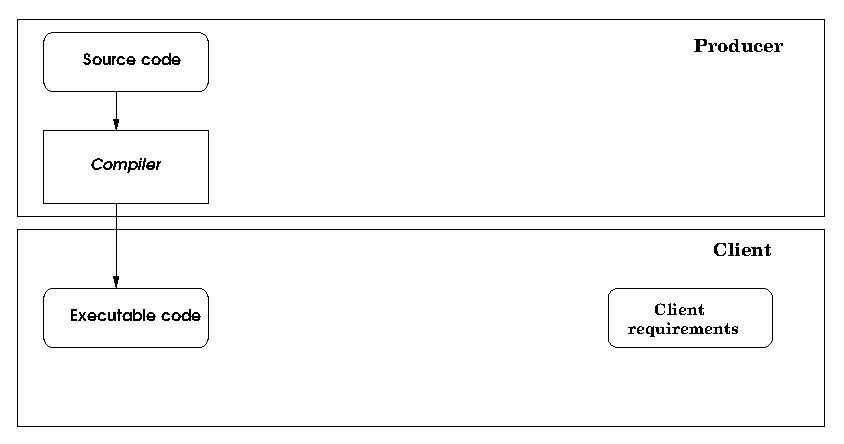
\epsfig{file=figs/mobileCode.eps}
% \end{center}
%  \end{frame}

% security trusted personal devices 
% are used for security sensitive applications, they manage confidential data
% and rely on limitted resources
\begin{frame}\frametitle{Security and trusted personal devices}
\begin{itemize}
\item Trusted personal devices: phones, smart cards, pda's, set
top boxes, \dots
\item Used for security-sensitive applications
\item Network connected
%\item Support for complex applications (contain a full JVM)
%\item Shift from hardware attacks to logical attacks
\end{itemize}
\end{frame}


\begin{frame}\frametitle{Mobile code and Java}
 % the de facto language for web applications , mobile phones, what ever smart cards
The defacto language for web applications:
 \begin{itemize}
  \item platform independent execution framework
  % \item  % With the JVM available in most popular browsers, the concept of mobile code was born. 
  \item widely used in   smart card applications
 \end{itemize}

Security guarantees: 
\begin{itemize}
    \item type safety,  bytecode verifier
     \item sandbox mechanism
\end{itemize}

But malicious code may use also 
\begin{itemize}
     \item logical attacks
     \item resource attacks
       \item information leaks
\end{itemize}
\end{frame}



\begin{frame}\frametitle{Guaranteeing security with formal verification}
  \begin{itemize}
    \item Specification language 
         \begin{itemize}
	    \item formalism for expressing program properties
	  \end{itemize}
    \item Program calculi for reasoning about program correctness 
       \begin{itemize}
	  \item reasoning directly on the operational semantics
	  \item Hoare logic  
	  \item Verification condition generators
       \end{itemize}
    \item Decision procedure 
        \begin{itemize}
	    \item automatic decision procedures
	    \item interactive theorem prover
	\end{itemize}
  \end{itemize}
\end{frame}


\begin{frame}[fragile,shrink]\frametitle{JML.Features}
  \begin{itemize}
     \item Contract based approach
             \begin{itemize}
	         \item preconditions
		 \item postconditions
	     \end{itemize}
       \item Class specification 
	 \begin{itemize}
	         \item object invariants
		 \item class history constraints
	     \end{itemize}
       \item Method annotations
	  \begin{itemize}
	         \item loop invariants 
		   \item assertions at particular program points
	    \end{itemize}

	         \item Special specification constructs  
	  \begin{itemize}
	         \item keywords \lstinline!\TYPE!, \lstinline!\result!
		 \item operators   \lstinline!\old!, \lstinline!\typeof!
		 \item ghost variables   \lstinline!//@ ghost int Memory!
	    \end{itemize}

  \end{itemize}

\end{frame}

\begin{frame}[fragile,shrink]\frametitle{JML.Example}
  \begin{lstlisting}[language=java]
//@ requires k >= 0 ;
//@ ensures \result == k*(k+1)/2;
public int sum (int k) {
  int sum = 0;		
  //@loop_modifies sum,i;
  //@loop_invariant i >= 0 && i<=k && 
  //@(sum == i*(i+1)/2);
  for  (int i = 0; i < k; i++ ) {
    sum = sum + i;
  } 	
  return sum;
}
\end{lstlisting} 
\end{frame}

 \begin{frame}\frametitle{Program calculi. Weakest precondition predicate transformers}
	% \begin{block}{Rules}
	   \begin{itemize}
	      \item handles possible side effects
		{\tiny $$ \wpSrcStmt{ \var = \expressionSrc_2}{\normalPostSrc }{ \excPostSrc } =
                  \wpSrcExpr{\expressionSrc_2 }{ 
				    \normalPostSrc \subst{\var}{v}   
				   }{ \excPostSrc}{v} 
		  $$ } 
	      \item exceptional termination 
		{\tiny $$   \begin{array}{l}  \wpSrcExpr{\expressionSrc.\fieldd  }{\normalPostSrc }{ \excPostSrc }{v}  = \\
	                        \wpSrcExpr{\expressionSrc }{%\\
			                  % \phantom{wpiSr} 
                                             %\begin{array}{l} 
						        v_1 \neq \Mynull \Rightarrow \normalPostSrc \subst{v}{v_1.\fieldd} %\\
			                                \wedge% \\
						        v_1 = \Mynull \Rightarrow%\\
							 %\Myspace 
							 %\left( \begin{array}{l} 
							      % \forall \freshVar, 
							     % \neg \instances(\freshVar) \wedge \\
							       %\freshVar \neq \Mynull \Rightarrow%\\ 
							       \excPostSrc(\NullPointerExc ) %\subst{\EXC}{\freshVar}
							 % \end{array}\right)
							        
		                                 % \end{array}
						   }{% \\ 
                                          % \phantom{wpiSrc}
					    \excPostSrc }{v_1}  
				\end{array} $$ }
	      
	  \end{itemize}
    %\end{block}
 \end{frame}


\begin{frame}[shrink]\frametitle{Architecture of a program verification tool}
\begin{center}
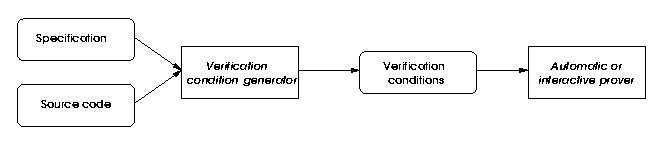
\epsfig{file=figs/sourceVerification.eps}
\end{center}

Several verification tools for Java exist:  The Loop tool, ESC/java, Krakatoa, Loop, Jive, the Key tool, JACK ...
\end{frame}



\begin{frame}\frametitle{History of JACK}
\begin{itemize}
\item Development started at Gemplus (Jan 2002 to April 2003)\\
Objective: Give developers tools that help them to provide and be
accountable for quality of their code
\begin{itemize}
\item Conform to specification requirements
\item Well-documented
\item Without bugs
\end{itemize}
\item Transfered to INRIA (September 2003)
\end{itemize}
\end{frame}



\begin{frame}\frametitle{Features of JACK}
\begin{itemize}
\item Tight integration with IDE Eclipse
\item JML used as annotation language
\item Support for Simplify (automatic) and Coq (interactive) prover
\item Special JACK view for verification condition browsing
\end{itemize}
\end{frame}


\begin{frame}\frametitle{Developing an application in Eclipse}
\vspace*{-1.5em}
\includegraphics[height=\textheight]{figs/screen1.ps}
\end{frame}

% source not sufficient
\begin{frame}\frametitle{However...}
  Source verification not always suitable
   \begin{itemize}
     \item in mobile code  scenarios, the client receives only executable code   
     \item software audit which does not trust the compiler
   \end{itemize}  
\end{frame}



\begin{frame}\frametitle{Motivation}
  \begin{itemize}
   \item How  to  bring to bytecode programs the benefit from source verification?
     \item How to check mobile code against complex functional policies? 
  \end{itemize}
\end{frame}


\begin{frame}[fragile, shrink]\frametitle{Proposal}
\begin{center}
\epsfig{file=figs/toolSetPCC.eps}
\end{center}
\end{frame}
%%%%%%%%%%%%%%%%%%%%%%%%%%%%%%%%%%%%%%%%%%%%%%CONTRIBUTIONS%%%%%%%%%%%%%%%%%%%%%%%%%%%%%%%%%%%%%%%%%%%%%%%%%%%%%%%%%%%%%%%%%%%%%%%%%%%%%%%%%%%%%%%%%%%%%%%%%%%%%%%%%%%%%%%%%%%%%%%%%


\begin{frame}\frametitle{Contributions}   
  \begin{itemize}
     \item Specification language for bytecode BML
     \item Compilation from source JML to BML specification
     \item Verification procedure for bytecode 
     \item Proof preserving compilation
\end{itemize}
\end{frame} 






%%%%%%%%%%%%%%%%%%%%%%%%%%%%%%%%%%%%%%%%%%%BML%%%%%%%%%%%%%%%%%%%%%%%%%%%%%%%%%%%%%%%%%



  \begin{frame}[shrink]\frametitle{BML.Design features}
   \begin{itemize}
      \item Corresponds to subset of JML
       \item  semantics - the same  as JML
     \item Java compiler independent
        \begin{itemize}
	    \item compilation process separate from Java compiler
	      
	  \end{itemize}
     \item Java Virtual Machine (JVM) compatibility 
       \begin{itemize}
	      \item compiled into user defined class attributes 
		 in compliance with the JVM specification
	  \end{itemize}     
      \item Syntax - does not support all the syntactic sugar in JML
   \end{itemize} 
\end{frame}



  \begin{frame}[shrink]\frametitle{BML. Restrictions}
   \begin{itemize} 
      \item Compiler 
	   \begin{itemize} 
               \item non optimizing compiler
	       \item not so restrictive as up to date most Java compilers 
		     do not perform optimizations
	   \end{itemize}
      \item Class file format
	 \begin{itemize} 
               \item \textbf{Line Number Table} - needed for identifying the exact points of the 
		 intra method specification
		 \item \textbf{Local Variable Table}  - needed for linking the names of method parameters
         \end{itemize}
   \end{itemize}
 \end{frame}

%%%%%%%%%%%%%%%%%%%%%%%%%Compiler from JML to BML%%%%%%%%%%%%%%%%%%%%%%%%%%%%

\begin{frame}[shrink]\frametitle{Compiler from JML to BML}
     
   Input : annotated  Java source and its corresponding class file
   Output : class file containing BML specification 
     \begin{itemize}
         \item annotated Java file 
          \item Compilation of the Java source file 
	    \item Compilation of ghost variables
	      \item Desugaring of JML specification
		\item Linking phase
		  \item Locating the points for intra method specification 
		    \item Encoding the BML specification into user defined class attributes
       \end{itemize}
\end{frame}


\begin{frame}[fragile,shrink]\frametitle{Example}
\begin{columns}
\begin{column}{5.1cm}
{\tiny
\begin{lstlisting}[language=java]
//@ requires k >= 0 ;
//@ ensures \result == k*(k+1)/2;
public int sum (int k) {
  int sum = 0;		
  //@loop_modifies sum,i;
  //@loop_invariant i >= 0 && i<=k && 
  //@(sum == i*(i+1)/2);
  for  (int i = 0; i < k; i++ ) {
    sum = sum + i;
  } 	
  return sum;
}
\end{lstlisting}}
\end{column}

\begin{column}{5.1cm}
{\tiny
\begin{lstlisting}[language=jvmis]
//@requires lv[1] >= 0;
//@ensures result == lv[1]*(lv[1] + 1)/2;
Loop specification
//@atIndex 14 
//@modifies  lv[2], lv[3]
//@invariant lv[3]>=0 && lv[3]<=lv[1] &&
//@    lv[2]==lv[3]*(lv[3]+1)/2
0 iconst_0
1 istore_2
2 iconst_0
3 istore_3
4 goto 14 
7 iload_2
8 iload_3
9 iadd
10 istore_2 
11 iinc 3 
14 iload_3
15 iload_1
16 if_icmplt 7 
19 iload_2
20 ireturn
\end{lstlisting}}
\end{column}
\end{columns}
\end{frame}

%%%%%%%%%%%%%%%%%%%%%%%%%%%%%%%%%VC gen%%%%%%%%%%%%%%%%%%%%%%%%%%%%%%%%%%%%%%%%%%%%%%
\section{Verification condition generator for Java bytecode}
\begin{frame}[fragile,shrink]\frametitle{Support} 
  \begin{itemize}
   \item Generates verification conditions for every method separately
   \item Works over the control flow graph of a method
   \item Support for object manipulation, exceptions, method invokations, stack manipulation
   \item Based on weakest precondition calculus
\end{itemize}

\end{frame}

\begin{frame}[fragile,shrink]\frametitle{Weakest precondition predicate transformer for bytecode}
\begin{definition}
   $$\wpi:  nat \rightarrow \Method  \rightarrow \Pred $$
\end{definition}


   $$ {\small \begin{array}{l}
        
      \frac{ \begin{array}{l}
	       \wpi(i+1,\methodd)\subst{\counter}{\counter+1} \subst{\stack{\counter + 1}}{\locVar{k}} \\
              \methodd[i] = \load \  \locVar{k}
             \end{array}
           }{\wpi(i,\methodd )} 
         
	 
	\\\\\\

      \frac{\begin{array}{l} 
                  \stack{\counter } \neq \Mynull \Rightarrow 
                            \wpi(i+1,\methodd)\subst{\stack{\counter}}{f(\stack{\counter} )} \ \wedge \\ 
			   
			     \stack{\counter } == \Mynull \Rightarrow \methodd.\excPost( i, \NullPointerExc) \\
                  \methodd[i] = \getfield \ f 
          \end{array}
     } { \wpi(i,\methodd ) }
        
      \end{array} } $$

\end{frame}

\begin{frame}[fragile,shrink]\frametitle{Correctness}
  \begin{definition} 
    If a method \methodd{} starts execution in state $s_0$, and terminates execution in $s_1$, i.e.  \ $\methodd: \  s_0 \rightarrow^{*} s_1 $ and
    $s_0 \vDash \methodd.Pre $ holds     then $s_1 \vDash \methodd.Post$
    \end{definition}
 
Assumption: 
\begin{itemize}
   \item reducible control flow graph 
\end{itemize}

\end{frame}



\begin{frame}[fragile,shrink]\frametitle{Example}
\begin{lstlisting}[language=jvmis]
method min((*@ \locVar{1} , \locVar{2}  @*) )
(*@\alert<7->{ \{ {\tiny $\locVar{1} \le \locVar{2} \wedge \locVar{1} > \locVar{2} \Rightarrow \locVar{1}  == \locVar{2} \wedge 
                          \locVar{1} > \locVar{2}    \wedge \locVar{1} \le \locVar{2} \Rightarrow \locVar{2} == \locVar{1} $} \}} @*)
   0: load 1
(*@\alert<6->{ \{ {\tiny $\stack{\counter } \le \locVar{2} \wedge \locVar{1} > \locVar{2} \Rightarrow \locVar{1}  == \locVar{2} \wedge 
                          \stack{\counter} > \locVar{2}    \wedge \locVar{1} \le \locVar{2} \Rightarrow \locVar{2} == \locVar{1} $} \}} @*)
   1: load 2
(*@\alert<5->{ \{ {\tiny $\stack{\counter - 1} \le \stack{\counter} \wedge \locVar{1} > \locVar{2} \Rightarrow \locVar{1}  == \locVar{2} \wedge 
                          \stack{\counter - 1} > \stack{\counter}    \wedge \locVar{1} \le \locVar{2} \Rightarrow \locVar{2} == \locVar{1} $} \}} @*)
   2: if_icmpgt 5
(*@\alert<4->{ \{ {\tiny $ \locVar{1} > \locVar{2} \Rightarrow \locVar{1}  == \locVar{2} \wedge 
		\locVar{1} \le \locVar{2} \Rightarrow \locVar{1} == \locVar{1} $} \}} @*)
   3: load 1
(*@\alert<3->{ \{ {\tiny $ \locVar{1} > \locVar{2} \Rightarrow \stack{\counter}== \locVar{2} \wedge 
		\locVar{1} \le \locVar{2} \Rightarrow   \stack{\counter} == \locVar{1} $} \}} @*)
   4: return
(*@\alert<2->{ \{ {\tiny $ \locVar{1} > \locVar{2} \Rightarrow \result == \locVar{2} \wedge 
		\locVar{1} \le \locVar{2} \Rightarrow \result == \locVar{1} $} \}} @*)

(*@\alert<4->{ \{ {\tiny $ \locVar{1} > \locVar{2} \Rightarrow \locVar{2}  == \locVar{2} \wedge 
		\locVar{1} \le \locVar{2} \Rightarrow \locVar{2} == \locVar{1} $} \}} @*)
   5: load 2
(*@\alert<3->{ \{ {\tiny $ \locVar{1} > \locVar{2} \Rightarrow \stack{\counter} == \locVar{2} \wedge 
		\locVar{1} \le \locVar{2} \Rightarrow \stack{\counter} == \locVar{1} $} \}} @*)
   6: return
(*@\alert<2->{ \{ {\tiny $ \locVar{1} > \locVar{2} \Rightarrow \result == \locVar{2} \wedge 
		\locVar{1} \le \locVar{2} \Rightarrow \result == \locVar{1} $} \}} @*)
\end{lstlisting}
\end{frame}


%%%%%%%%%%%%%%%%%%% Proof preserving compilation %%%%%%%%%%%%%%%%%%%%5

\section{Proof preserving compilation}

\begin{frame}\frametitle{Compiler}

       \begin{itemize}
           \item Non - optimizing 
           \item Targets a stack based virtual machine
	   %\item close to standard Java compilers 
       \end{itemize}
       Not so bad as  most of the Java compilers today are non optimizing  and  the result is relevant for the JVM 
 \end{frame}



\begin{frame}[fragile,shrink]\frametitle{Equivalence of proof obligations.Example}

\begin{block}
  {\small \begin{tabular}{lll} 
   $ \compileLabel{i}{ \lstinline!sqr + 2*s ! }{i+4}$ & = &
   \begin{tabular}{l} 
     $\compileLabel{i}{ \lstinline!sqr! }{i}$ \\
     $\compileLabel{i+1}{ \lstinline!2*s! }{i+3} $\\
     \lstinline!i+4: add!
      \end{tabular} \\
      where & & \\
      $\compileLabel{i}{ \lstinline!sqr! }{i}$ & = & \lstinline! i: load sqr!\\
      \\
      $\compileLabel{i+1}{ \lstinline!2*s! }{i+3}$ & = &
      \begin{tabular}{l} 
        % \lstinline!i  : load sqr! \\
	 \lstinline!i+1: const 2!  \\
	 \lstinline!i+2: load s!   \\
	 \lstinline!i+3: mul!	   \\
	 %\lstinline!i+4: add!	    
   \end{tabular}
    \end{tabular}
}
\end{block}


%\begin{block}
  {\small
  $$  \begin{array}{ll}
         1.1   &     \alert<7->{ \mbox{\rm \lstinline!sqr!} + \mbox{\rm \lstinline!2!}*\mbox{\rm \lstinline!s!} = \mbox{\rm \lstinline!5!}   } \\ 
         1.2   &   \lstinline!i:  load sqr!  \\
         1.3   &     \alert<6->{  \stack{\counter} + \mbox{\rm \lstinline!2!}*\mbox{\rm \lstinline!s!} = \mbox{\rm \lstinline! 5!}   }\\
         1.4   &   \lstinline!i+1: const 2!	  \\
	 1.5   &     \alert<5->{   \stack{\counter - 1} + \stack{\counter } *\mbox{\rm \lstinline!s!} = \mbox{\rm \lstinline! 5!}    }\\
	 1.6   &   \lstinline!i+2: load s!	  \\
	 1.7   &     \alert<4->{   \stack{\counter - 2}  + \stack{\counter - 1} * \stack{\counter} = \mbox{\rm \lstinline! 5!}    }\\
	 1.8   &   \lstinline!i+3: mul!	          \\
	 1.9   &     \alert<3->{  \stack{\counter - 1}  + \stack{\counter} = \mbox{\rm \lstinline! 5!}   }\\
	 1.10  &   \lstinline!i+4: add!	          \\
	 1.11  &     \alert<2->{  \stack{\counter} = \mbox{\rm \lstinline! 5 !}    } \\       
               & \\
	       & \\
  %\end{array}$$}

%\end{block}



  % \begin{Example} {
  %{\small $$\begin{array}{ll}
      2.1   &    \wpSrcExpr{\lstinline!sqr + 2*s ! }{\alert<2->{ v = 5} }{\excPostExpl}{v} =   \\
      2.2   &  	 \wpSrcExpr{\lstinline!sqr!}{\wpSrcExpr{\lstinline!2*s ! } { \alert<3->{ (v=5)\subst{v}{v_{sqr} + v_{2*s}} } }{\excPostExpl}{v_{2*s}}  }{\excPostExpl}{v_{sqr}} =   \\
      2.3   & 	 \wpSrcExpr{\lstinline!sqr!}{\wpSrcExpr{\lstinline!2! }{\wpSrcExpr{\lstinline!s! }{ \alert<4->{ (v_{sqr}+v_{2*s}=5)\subst{v_{2*s}}{v_{2}*v_{s}}} }{\excPostExpl}{v_{s}}  }{\excPostExpl}{v_{2}} }{\excPostExpl}{v_{sqr}} =   \\
      2.4   &	 \wpSrcExpr{\lstinline!sqr!}{\wpSrcExpr{\lstinline!2! }{\alert<5->{ (v_{sqr} + v_{2}*v_{s}=5 ) \subst{v_{s}}{s}} }{\excPostExpl}{v_{2}} }{\excPostExpl}{v_{sqr}} =   \\
      2.5   &    \wpSrcExpr{\lstinline!sqr!}{\alert<6->{(v_{sqr} + v_{2}*\lstinline!s!=5 ) \subst{v_{2}}{2} } } {\excPostExpl}{v_{sqr}} =   \\
      %2.6   &	 (v_{sqr} + 2*\lstinline!s!=5 ) \subst{v_{sqr}}{\lstinline!sqr!  } =   \\
      2.6   & \alert<7->{  \lstinline!sqr! + 2*\lstinline!s!=5  }
\end{array}$$
} %}  \end{Example}

\end{frame}


%%%%%%%%%%%%%%%%%%%%%%%%%%%%%%%%%%%APPLICATIONS %%%%%%%%%%%%%%%%%%%%%%%%%%%%%%%%%%%%%
 \section{Applications}
%%%%%%%%%%%%%%%%%%%%%%%%%%%%%%%%%%%Java To native compilation%%%%%%%%%%%%%%%%%%%%%%%%%%%%%%%%%%%%%
 
 \subsection{Java-to-Native Compilation}

\begin{frame}[shrink]\frametitle{Java-to-Native Compilation}
 Compiling Java bytecode into native code brings runtime advantages:
\begin{itemize}
    \item Faster execution
    \item Especially beneficial for restrained systems with non-sophisticated JVMs
\end{itemize}
But Java-to-Native compilation also comes with a drawback:
\begin{itemize}
    \item Native code is typically 3 to 4 times bigger than bytecode,
\end{itemize}
\end{frame}

\begin{frame}[fragile]\frametitle{Why is Native Code so Huge? An Example}
The \emph{idiv} bytecode throws an \texttt{ArithmeticException} if the divisor is equal to zero:

\begin{columns}
\begin{column}{5.1cm}
\begin{lstlisting}[language=jvmis]
iload i
iload j
idiv
ireturn
\end{lstlisting}
\end{column}
\begin{column}{5.1cm}
\begin{lstlisting}[language=C]
int i, j;
 \alert{if (j == 0)}
   \alert{THROW(ArithmeticException);}
RETURN_INT(i / j);
\end{lstlisting}
\end{column}
\end{columns}
\bigskip
There are many checks of this kind:
\begin{itemize}
\item Checking a pointer is not \emph{null} before dereferencing it,
\item Checking an array is accessed inside its bounds,
\item Checking an array is created with a positive size,
\item Checking affected types are compatible,
\item ...
\end{itemize}
SPECjvm98: 2964 exception check sites for a native size of 23598 bytes (Ishizaki et al.).
\end{frame}


\begin{frame}\frametitle{Suppressing Exceptions Check Sites using formal verification}

Runtime exceptions are (usually) a safety against programming errors. They should not be triggered by sane code.

We propose to formally prove that runtime exceptions are never thrown by a program.

Methodology:
\begin{enumerate}
\item Annotate source code with JML specification to express that no runtime exception will be thrown
\item Compile JML specification into BML as user-defined class file attributes
\item Generate and prove verification conditions over the bytecode and BML
\item Annotate class files with useless runtime exception check sites attribute
\end{enumerate}
\end{frame}

\begin{frame}
\frametitle{Experimental Results}
\begin{center}
  Number of necessary exception check sites

  \bigskip
  \begin{tabular}{|l|r@{\extracolsep{0.2cm}}rr|}
    \hline
    \multirow{2}*{Program} & \multicolumn{3}{c|}{\# of exception check sites} \\
    \cline{2-4} & Bytecode & ~~~~~~JC & Proven AOT\\
    \hline
    \benchname{crypt} & 190 & 79 & 1\\
    \benchname{banking} & 170 & 12 & 0\\
    \benchname{scheduler} & 215 & 25 & 0\\
    \benchname{tcpip} & 1893 & 288 & 0\\
    \hline
  \end{tabular}
  \bigskip
  \begin{tabular}{|l|r@{\extracolsep{0.2cm}}rr|}
    \hline
    \multirow{2}*{Program} &  \multicolumn{3}{c|}{Memory footprint (bytes)}\\
    \cline{2-4} & Bytecode & Native AOT & Proven AOT\\
    \hline
    \benchname{crypt} & 1256 & 5330 & 1592\\
    \benchname{banking} & 2320 & 5634 & 3582\\
    \benchname{scheduler} & 2208 & 5416 & 2504\\
    \benchname{tcpip} & 15497 & 41540 & 18064\\
    \hline
  \end{tabular}
\end{center}
\end{frame}

% \begin{frame}
%\frametitle{The good and the bad news}
%\begin{itemize}
% \item The ratio between the bytecode and the proven native code is smaller than 2 
% \item Methodology - suitable for closed system. If a new system composant is added the whole system must be reverified
%\end{itemize}
%\end{frame}

\subsection{Constraint memory consumption policies using BML}
 
\begin{frame} \frametitle{Problem}

     \begin{itemize} 
        \item smart card devices, embedded devices, TPDs have limitted computational resources
	  \item vulnerable to denial of service attacks. 
	    \item need of mechanisms for guaranteeing that an application 
	      respects the limitation of the device
   \end{itemize}
\end{frame}

\begin{frame}[containsverbatim] \frametitle{Modeling the memory heap}  
  \begin{block}<+->{Used heap space is a ghost variable}
    \begin{verbatim} //@ public ghost static int Mem \end{verbatim}
  \end{block}
  

  \begin{block}<1->{ The upper bound of the memory space that can be used is a model variable}
    \begin{verbatim} //@ public ghost static int Max \end{verbatim}   
  \end{block}
\end{frame}


\begin{frame}[containsverbatim,shrink] \frametitle{Principles for specifying memory allocations}
  \begin{Example} {
    \begin{lstlisting}[language=jvmis]
      method m
         new A
         //@set Mem = Mem+memUnit(A)
         dup
         invokevirtual A
    \end{lstlisting}
 }   
  \end{Example} 
  
  \begin{block}<+->{The $wp$ rule for the set specification construction }
     $wp(\verb!set Mem = M! , \psi , \psi') = \psi[\verb!Mem! \leftarrow \verb!M!] $
  \end{block}
\end{frame}

\begin{frame} \frametitle{Specifying methods}
  \begin{block}<+->{Method Specification}
    \begin{itemize}
      \item  <1->{ expresses the fact that the method does not break the bounded memory consumption policy }
      
      \item  <2->{  assume in the precondition that  when method starts execution the application has consumed so much memory units such that the method execution 
 will not break the memory consumption restrictions}
      \item  <3->{ guarantee postcondition -  when method ends execution it should have consumed not more than what it has assumed in the precondition  }
     \end{itemize}
  \end{block}
\end{frame}

\begin{frame}[fragile,shrink]\frametitle{Principles. Specifying Methods}
  \begin{Example}{
      \begin{lstlisting}[language=jvmis]
      //@requires Mem+memUnit(A)+
      //@            methCons(init_A)<=Max
      //@ensures Mem<=old(Mem)+
      //@           memUnit(A)+methCons(init_A)
      method m
         new A
         //@set Mem = Mem+memUnit(A)
         dup
         invokevirtual A
      \end{lstlisting}         
       }
  \end{Example} 
\end{frame}


\begin{frame}[fragile,shrink]\frametitle{Principles. Loops}
 \begin{Example}{ {\tiny 
 \begin{lstlisting}[language=jvmis]
//@requires Mem + iter*( memUnit(A) + methCons(init_A)) <= Max
//@ensures Mem <= \old(Mem) +   iter*(memUnit(A) +  methCons(init_A))   
 method m(int iter)
  //@ghost int MemL
  //@set MemL = Mem
  Loop specification
  (*@\textsf{atIndex:}@*)16
  (*@\textsf{modifies}:@*)Mem, i
  (*@\textsf{invariant}:@*) Mem <= MemL + i*(memUnit(A) + methCons(init_A)) && i <= iter
  (*@\textsf{variant:}@*) iter-i
  0 const 0
  1 store i
  2 goto 16 
  5 new A
  //@set Mem=Mem+memUnit(A);
  8 dup
  9 invokespecial init_A
  12 store a
  13 iinc i
  16 load i
  17 load iter
  18 if_icmplt 5 
  21 return
 \end{lstlisting}}  
}\end{Example} 
\end{frame}



 
\section{Results}

\begin{frame}[fragile,shrink]\frametitle{What has been done?}
\begin{center}
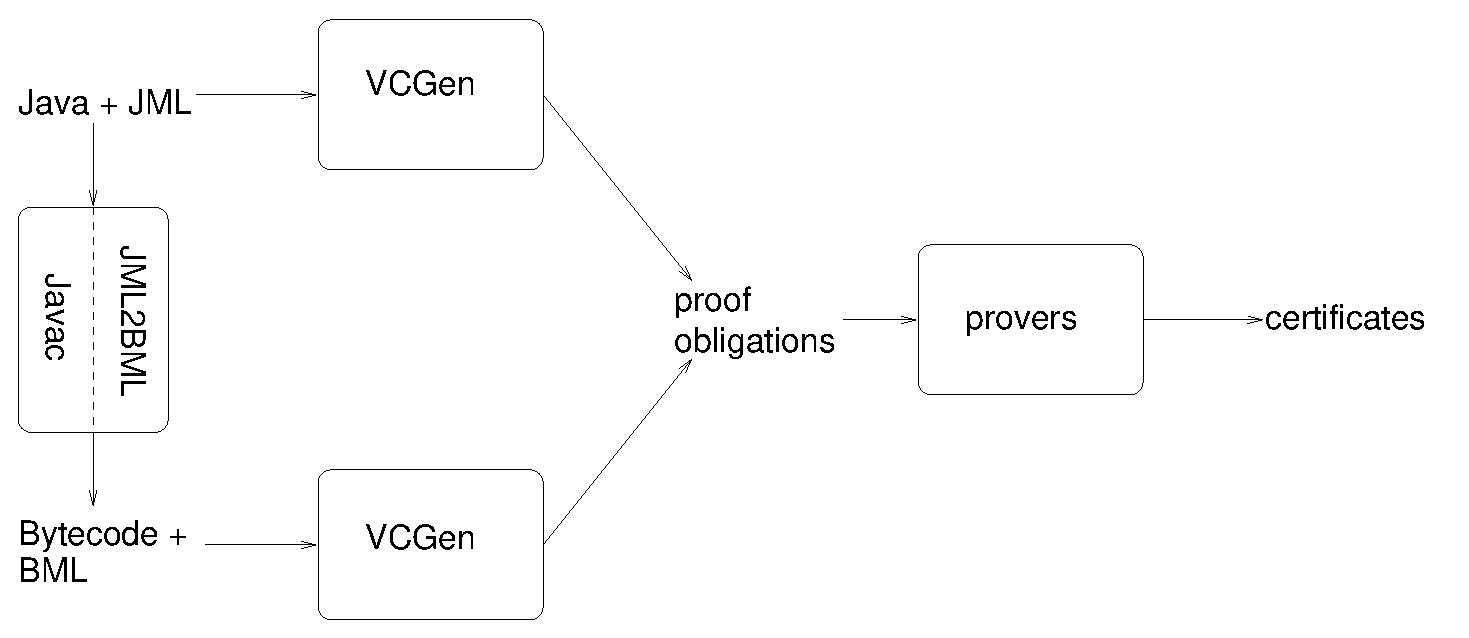
\includegraphics[height=\textheight]{figs/toolset.eps}
\end{center}
\end{frame}


 \section{Future work}

\begin{frame}[fragile,shrink]\frametitle{Towards  a PCC }
  Still missing the certificate. Desirable properties
                    \begin{itemize}
	                \item  small 
			  \item easily checked 
			  \item  hybrid certificates 
		     \end{itemize}

\begin{center}
\includegraphics{figs/toolSetPCC.eps}
\end{center}
\end{frame}


\begin{frame}[fragile,shrink]\frametitle{Future directions. Verification condition generator }
         \begin{itemize}	   
	    \item Extension of the verification condition generator 
                 \begin{itemize}
	             \item multithreading
		  \end{itemize}
           \item Machine checked proof
                 \begin{itemize}
	             \item reliable
		       \item important for a PCC framework
		  \end{itemize}
          \end{itemize}
\end{frame}




\begin{frame}[fragile,shrink]\frametitle{Future directions. Property coverage  }
	   
                  \begin{itemize}
	                \item pure methods 
			  \item alias control
			  \item modular verification of class invariants
			    
		   \end{itemize}  

\end{frame}


\section{Related work}

\begin{frame}[fragile,shrink]\frametitle{Related Work. Low level verification}


 \begin{itemize}
   \item The Spec\# programming system

     \item Peter Muller and Barnwatt

     \item Nipkow Wildmoser

      \item  The Grail project 
\end{itemize}

\end{frame}

\begin{frame}[fragile,shrink]\frametitle{ Relation between compiled and source code}
\begin{itemize}
   \item G.Barthe, T.Rezk A.Saabas - Proof Preserving Compilation 

 \item Peter Muller and Barnwatt - Translating Source Logic derivation  into bytecode derivation trees 


\item  C.Kunz, G.Barthe T.Rezk, B.Gregoire - Transforming annotations and proofs from source to optimized bytecode

 \end{itemize}

\end{frame}





\end{document}

